\newpage
\appendix
\section{Decision boundaries in the Long and Servedio experiment}
\begin{figure}[htp]
\centering
  \begin{subfigure}{0.31\linewidth}
    \includegraphics[width=\columnwidth]{figs/boundaries_Logistic.png}
    \subcaption{Logistic}
    \label{fig:logistic}
  \end{subfigure}
  \hfill
  \begin{subfigure}{0.31\linewidth}
        \includegraphics[width=\columnwidth]{figs/boundaries_Huberised.png}
    \subcaption{Huberised}
    \label{fig:huber}
  \end{subfigure}
  \hfill
  \begin{subfigure}{0.31\linewidth}
        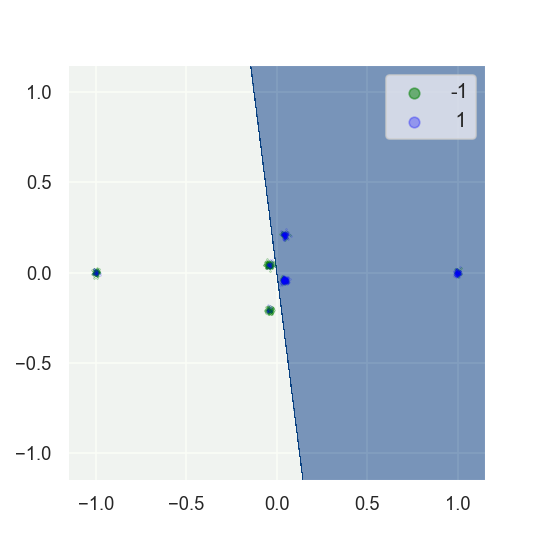
\includegraphics[width=\columnwidth]{figs/boundaries_Partial_Huberised.png}
    \subcaption{Partially Huberised}
    \label{fig:phuber}
  \end{subfigure}
  \caption{Decision boundaries in the reproduced \textcite{long_random_2010} experiment, with label noise flip probability $\rho = 0.2$. The logistic and Huberised logistic loss misclassify samples generated from the two \emph{penalizer} Gaussians centered around $\pm(\gamma, -\gamma)$, resulting in $50\%$ test accuracy. The partially Huberised logistic loss does not succumb to label noise, achieving near-perfect discrimination.}
  \label{fig:syntheticboundaries}
\end{figure}

\section{Effect of the label noise seed on the real-world experiments}
In the original paper \parencite{menon_can_2019}, all trials use the same corrupted dataset for each flip probability $\rho$. \autoref{tab:seed-results} shows the results obtained on a subset of our experiments when varying the random seed used to generate label noise.

\begin{table*}[htpb]
 \centering
 \resizebox{\textwidth}{!}{
\begin{tabular}{p{3em}ll|llll|p{4.5em}}
\toprule
\textbf{Label noise} & \textbf{Dataset} &\textbf{Loss function} &   Seed 0  &   Seed 1  &   Seed 2  &  Seed 3  & Original paper\\
\midrule
\multirow{6}{*}{$\rho = 0.6$} & \multirow{2}{*}{MNIST} & CE & 98.0 $\pm$ 0.1 &  97.9 $\pm$ 0.0 &  97.9 $\pm$ 0.0 &  97.9 $\pm$ 0.1 & 91.1  $\pm$  0.6 \\
& & PHuber-GCE  &  98.0 $\pm$ 0.0 &  97.8 $\pm$ 0.1 &  98.0 $\pm$ 0.0 &  98.0 $\pm$ 0.0 & 97.8 $\pm$ 0.0 \\
\cline{2-8} \rule{0pt}{10pt}
& \multirow{2}{*}{CIFAR-10 } & CE & 44.0 $\pm$ 0.2 &  43.8 $\pm$ 0.5 &  44.1 $\pm$ 0.2 &  43.2 $\pm$ 0.3 & 40.6 $\pm$ 0.3 \\
& & PHuber-GCE &  54.3 $\pm$ 0.5 &  54.0 $\pm$ 0.7 &  53.7 $\pm$ 0.5 &  54.3 $\pm$ 0.2 & 62.6 $\pm$ 0.2 \\
\cline{2-8} \rule{0pt}{10pt}
& \multirow{2}{*}{CIFAR-100 } & CE & 26.7 $\pm$ 0.1 &  27.1 $\pm$ 0.1 &  27.0 $\pm$ 0.5 &  26.9 $\pm$ 0.1 & 11.4 $\pm$ 0.2 \\
& & PHuber-GCE &  42.2 $\pm$ 0.4 &  43.0 $\pm$ 0.2 &  42.1 $\pm$ 0.6 &  41.9 $\pm$ 0.1 & 31.5 $\pm$ 0.8\\
\bottomrule
\end{tabular}
}
\caption{Impact of the random seed used to generate label noise. The mean and standard error of the test accuracy over 3 trials is reported. This subset of experiments was chosen to include both a baseline and a partially Huberised loss, at the highest level of label noise. The results obtained are consistent across seeds, and differ from the original paper's results.}
  \label{tab:seed-results}
\end{table*}
